\chapter{A Lesson in Lying}

This lecture begins by returning to unfinished business in Kant's moral theory and then turns, by a clear reset, to Kant's political theory and Rawls's hypothetical contract. We move from duty and autonomy, to the two standpoints from which morality becomes possible, to the hardest case of lying, and finally to the question of how contracts bind and when they justify.

\section{Duty, Autonomy, and Dignity}

Sandel opens by asking us to recover Kant's answer to a difficulty left over from the previous discussion. Duty seems to bind; autonomy seems to liberate. How can they possibly go together? The answer he draws from the class is simple in form and deep in consequence: duty is not obedience to an alien command if the moral law is one we impose on ourselves.

\begin{equation}
\text{duty} + \text{self-imposed law} \Longrightarrow \text{autonomy}
\end{equation}

The point is not merely that we happen to accept a rule. The point is that the will is governed by a law that it can acknowledge as its own. On this picture, freedom is not the absence of law. Freedom is lawgiving of a special kind.

Sandel immediately sharpens the point. Our dignity does not come from the mere fact that we answer to moral law. If that were all, dignity would consist in subjection. Kant's stronger claim is that dignity belongs to us insofar as we are authors of the law to which we are subject.

\begin{equation}
\text{author of the law} \Longrightarrow \text{dignity}
\end{equation}

This is the first structural move of the lecture. We do not begin with consequences, psychology, or social effects. We begin with the form of willing. That priority will govern the entire discussion that follows, especially when Sandel turns to lying.

\section{One Moral Law and Two Standpoints}

The first answer immediately generates a second question. If each of us gives the law to ourselves, why should there be one law rather than many? Why should my conscience coincide with yours?

\subsection{Question \& Answer}

The question is: if moral law is self-legislated, why does Kant not collapse into subjectivism?

Sandel's answer, prompted by the class, is that the relevant chooser is not the private empirical self. It is reason, and more precisely pure reason. The law is universal because the faculty that legislates it is not contingent on my desires, your upbringing, or anyone's special social position.

\begin{equation}
\text{pure reason shared by all} \Longrightarrow \text{one universal moral law}
\end{equation}

This resolves one tension only by opening a larger one. Even if we grant that autonomy and universality can go together, how is a categorical imperative possible at all? How can morality be more than inclination dressed up in noble language?

Sandel answers by introducing the distinction between two standpoints.

\begin{align}
\text{sensible world} &\Longrightarrow \text{nature, cause and effect}, \\
\text{intelligible world} &\Longrightarrow \text{autonomy, self-given law}.
\end{align}

As objects of experience, we belong to the sensible world. There our actions can be described by the ordinary language of nature: causes, effects, appetites, pain, pleasure, and the rest. But as subjects of experience, we can also regard ourselves from another standpoint, the intelligible world, where freedom is possible.

\begin{figure}[h]
\centering
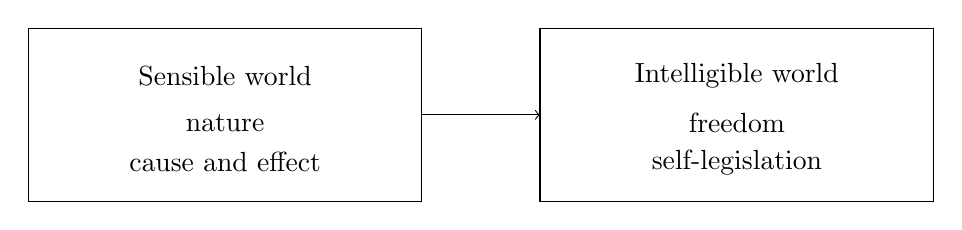
\begin{tikzpicture}[x=1cm,y=1cm]
\draw (0,0) rectangle (5,2.2);
\node at (2.5,1.6) {Sensible world};
\node at (2.5,1.0) {nature};
\node at (2.5,0.5) {cause and effect};

\draw (6.5,0) rectangle (11.5,2.2);
\node at (9,1.6) {Intelligible world};
\node at (9,1.0) {freedom};
\node at (9,0.5) {self-legislation};

\draw[->] (5,1.1) -- (6.5,1.1);
\end{tikzpicture}
\end{figure}

This is not a decorative metaphysical distinction. It is the framework within which the possibility of morality is to be understood. If we were wholly empirical beings, then every exercise of will would be conditioned by some desired object. Choice would then be heteronomous all the way down.

\begin{equation}
\text{empirical being only} \Longrightarrow \text{heteronomy} \Longrightarrow \neg \text{freedom}
\end{equation}

From this standpoint the critique of utilitarianism becomes visible. If the human person is understood solely through the calculus of pleasure, pain, appetite, and satisfaction, then freedom disappears. What remains is a refined mechanism of desire.

\subsection{Question \& Answer}

The question is: how can we be determined by nature and still be free?

Sandel's answer is that we occupy both standpoints at once. As empirical beings we are subject to necessity. As rational agents we can regard ourselves as capable of autonomy. The moral life is possible precisely because these two descriptions do not collapse into one another.

\begin{equation}
\text{inhabit both realms} \Longrightarrow \text{gap between is and ought}
\end{equation}

That is why the lecture insists that morality cannot be read off from science. Science tells us what is the case in the empirical world. It does not settle what ought to be done.

\begin{equation}
\text{morality} \neq \text{empirical science}
\end{equation}

\section{The Murderer at the Door}

Having built the formal structure, Sandel now subjects it to the hardest test he can find. Kant says lying is wrong. Benjamin Constant objects that this absolute prohibition cannot be right. Suppose a murderer comes to the door asking for a friend hidden in the house. Surely one should lie.

Kant's reply, as Sandel presents it, is severe but consistent. Once we allow consequences to carve out exceptions to the categorical imperative, the entire framework changes. We are no longer doing Kantian ethics. We are doing some form of consequentialism.

\begin{equation}
\text{lie} \Longrightarrow \text{violation of the categorical imperative}
\end{equation}

At this point Sandel does not soften the problem. He deepens it. He asks whether there is some way to avoid lying without surrendering the friend. This is the important pedagogical turn. The lecture does not move from principle straight to conclusion. It moves from principle to experiment.

The first experiment is unsatisfactory. One may try to arrange matters so that a statement that sounds deceptive later becomes literally true. Sandel treats this as too clever and not obviously Kantian. The second experiment is stronger: one may answer, ``I do not know where he is,'' where the sentence is strictly true at the instant of utterance, though designed to mislead. Now the real distinction comes into view.

\section{Lie, Misleading Truth, and the Moral Law}

The next movement of the lecture isolates a distinction that feels morally unstable at first hearing but is central to Sandel's defense of Kant. A lie is false. A misleading truth is true, though crafted so that the listener will draw the wrong conclusion.

\begin{equation}
\text{lie} \neq \text{misleading truth}
\end{equation}

Why should this matter if the expected consequences are much the same? Sandel's answer is that Kant does not base morality on consequences. The relevant difference lies in the formal relation of the act to the moral law.

A small social example makes the point less dramatic. Someone gives us an ugly tie and asks what we think. A white lie would be to say it is beautiful. A misleading truth would be to say that we have never seen a tie like it before. The surface triviality of the example is useful. It lets the structure appear without the pressure of the murderer case.

Sandel then turns to the Clinton example because it forces the same issue into public speech. Was the statement merely evasive, or was it a lie? The class exchange here is crucial, because it lets Sandel draw the contrast between outcome and motive more sharply than the earlier examples allowed.

\subsection{Question \& Answer}

The question is: if both statements aim at deception, why is a misleading truth not morally equivalent to a lie?

The class objection, voiced through Wesley, is that in both cases the motive seems to be the same: to mislead. Sandel answers by distinguishing the hoped-for effect from the form of the act itself. In the case of the misleading truth, the speaker still keeps faith, however imperfectly, with the requirement to speak truly.

\begin{equation}
\text{misleading truth}
\Longrightarrow
\text{truth spoken} + \text{intended evasion} + \text{homage to duty}
\end{equation}

This formula is schematic rather than textual, but it captures the lecture's point. Sandel's claim is not that the evasive speaker is innocent. It is that the evasive speaker pays a certain homage to duty by refusing outright falsehood. That homage is precisely what is absent in the lie.

A short derivation makes the logic clear.

\begin{enumerate}
\item A lie violates truth at the level of utterance.
\item A misleading truth preserves truth at the level of utterance.
\item Kant judges acts by their conformity to the moral law, not by consequences alone.
\item Therefore the two acts are not formally identical, even when they aim at similar results.
\end{enumerate}

This is also why Sandel returns, at the end of the exchange, to the thought that consequences are not under our control in the decisive way. We may hope the murderer is deceived, but what we can control is whether we ourselves speak falsely.

\section{Kant's Political Theory and Rawls's Original Position}

At this point the lecture resets. Sandel says, in effect, that we have been discussing Kant's application of the categorical imperative to lying, and now we turn to another application: political theory.

Kant, as Sandel presents him, is a contractarian, but of a very special kind. Just laws arise from social contract only if the contract is not treated as an actual bargain among historically situated persons with competing interests and unequal advantages. The contract that matters is an idea of reason.

\subsection{Question \& Answer}

The question is: what moral force can a hypothetical contract have if no one actually signed it?

Sandel's answer begins negatively. An actual constitutional convention does not automatically generate justice because actual persons bring with them unequal bargaining power, special interests, and unequal knowledge. Agreement by itself does not purify those asymmetries.

\begin{equation}
\text{actual contract} \not\Longrightarrow \text{just terms}
\end{equation}

The hypothetical contract matters precisely because it abstracts from those contingencies. Sandel then introduces Rawls as the thinker who develops this Kantian strategy in detail. Rawls shares Kant's anti-utilitarianism and gives the hypothetical contract its operational form through the veil of ignorance and the original position.

\begin{align}
\text{veil of ignorance} &\Longrightarrow \text{original position of equality}, \\
\text{hypothetical contract among equals} &\Longrightarrow \text{principles of justice}.
\end{align}

The movement here is from a moral idea to a device of construction. If we bracket race, class, health, talent, strength, weakness, and place in society, then the principles chosen under those conditions may plausibly claim to be principles of justice rather than the victory of one social position over another.

This part of the lecture remains preparatory. Sandel does not yet derive Rawls's principles. He first asks what any contract, real or hypothetical, can do morally.

\section{Actual Contracts, Reciprocity, and the Limits of Consent}

To answer the question about hypothetical contracts, Sandel turns back to actual contracts. He distinguishes two issues that are often run together: first, how contracts bind; second, whether they justify the terms they produce.

The first issue yields the lecture's most compact piece of moral architecture. Actual contracts have force in two ways.

\begin{align}
\text{consent} &\Longrightarrow \text{self-imposed obligation}, \\
\text{benefit received} &\Longrightarrow \text{reciprocal obligation}.
\end{align}

The lobster example is the cleanest worked case. I promise to pay \$100 if someone harvests and brings me 100 lobsters. The lobsters arrive; I consume the benefit; then I refuse to pay. Why am I obligated? Sandel presses the class until the point becomes plain: the strongest argument here is reciprocal benefit.

\paragraph{Worked example: the lobster cases.}

\begin{enumerate}
\item Case 1: agreement, performance, and benefit are all present.
\item The other party has worked on my behalf.
\item I have received and enjoyed the benefit.
\item Therefore an obligation arises even before we ask any deeper question about consent.
\end{enumerate}

Then Sandel alters the example. We make the same agreement, but I cancel it two minutes later, before any work is done and before any benefit has been conferred. Now reciprocity is missing. If obligation remains, it must arise from another source. This is where Adam's intervention matters: the promise may bind because the obligation was self-imposed.

\subsection{Question \& Answer}

The question is: is consent necessary for obligation, or can reciprocal benefit bind us even without agreement?

Sandel's answer is that neither simple formula is adequate. Consent can bind because it expresses autonomy. Benefit can bind because reciprocity has moral force. But the two do not always coincide, and neither is sufficient in every case to establish justice.

This is why the later examples matter. The baseball card case and the widow with the plumber show that actual agreement does not guarantee fairness. The Hume case and the repair-van case show that benefit can generate claims even where no explicit consent was given. The marriage examples are used to separate the two strands further: promise isolates consent; faithful performance isolates reciprocity.

The lecture's conclusion in this section is compact enough to state schematically.

\begin{equation}
\text{moral force of actual contracts} = \text{autonomy} + \text{reciprocity}
\end{equation}

But the equality sign must be read with care. This is not algebra. It is a structural decomposition. Real contracts often fail to realize either ideal cleanly.

\begin{align}
\text{power asymmetry} &\Longrightarrow \text{autonomy imperfectly realized}, \\
\text{knowledge asymmetry} &\Longrightarrow \text{reciprocity imperfectly realized}.
\end{align}

From here the return to Rawls is immediate. If we imagine a contract under conditions where power and knowledge are equalized, then the ideals that give contracts their moral force can be modeled without distortion.

\begin{equation}
\text{equal power} + \text{equal knowledge} \Longrightarrow \text{fair hypothetical agreement}
\end{equation}

That is the point of the veil of ignorance. It is not a historical story. It is a device for removing the contingencies that spoil the moral authority of actual bargains.

\section{Summary}

The lecture begins with Kant's moral theory and ends by setting up Rawls's theory of justice. Along the way it establishes a sequence of linked claims. Duty can be autonomous because the moral law is self-imposed. Universality is possible because the relevant legislator is pure reason rather than private preference. Morality requires a standpoint beyond the empirical order of appetite and causation. The prohibition on lying remains severe, but Sandel tries to rescue a distinction between lie and misleading truth by appealing to formal fidelity to duty. Finally, the force of contract is split into two distinguishable ideals, autonomy and reciprocity, neither of which is perfectly realized in ordinary social life.

The payoff is forward-looking. If actual contracts are morally forceful but not self-justifying, then justice must be sought from the standpoint of a hypothetical contract among equals. What principles would such a contract choose? That is the question left for the next lecture.